\documentclass[11pt,oneside]{article}
\usepackage[utf8]{inputenc}  
\usepackage[T1]{fontenc}
\usepackage{amsmath,amssymb,bm}
\usepackage{titlesec}
\usepackage{titletoc}
\usepackage{graphicx}
\usepackage[margin=2.5cm]{geometry}
\usepackage[frenchb]{babel}
\usepackage{hyperref}
\AddThinSpaceBeforeFootnotes
\FrenchFootnotes
\usepackage{ae,lmodern}
\usepackage{sectsty}
\usepackage[usenames,dvipsnames]{xcolor}
\usepackage{enumitem}
\usepackage{caption}
\usepackage{multicol}
\usepackage{pifont}
\usepackage{fancyhdr}
\pagestyle{fancy}
\fancyhf{}
\rhead{Rapport}
\lhead{\leftmark}
\rfoot{Page \thepage}
\renewcommand{\headrulewidth}{2pt}
\renewcommand{\footrulewidth}{1pt}
\definecolor{Rapport}{RGB}{213,25,50}
\definecolor{airforceblue}{rgb}{0.36, 0.54, 0.66}
\definecolor{amber}{rgb}{1.0, 0.75, 0.0}
\sectionfont{\bfseries\color{Plum}\LARGE}
\subsectionfont{\color{Mulberry}}
\parskip=10pt
\setlength{\parindent}{1cm}
\usepackage{comment}
\begin{document}
\begin{titlepage}
\phantom{aaaaaaaaaaaaaaaaaaaaaaaaaaaaaaaaaaaaaaa
ytrfdytfugvghikuhjbiujbhaaaaaaaaaaaaaaa}


\begin{minipage}[c]{.46\linewidth}
		\centering
		
\includegraphics[scale=0.1]{logo} 
	\end{minipage}
\hfill%
\begin{minipage}[c]{.46\linewidth}
		\centering
		
\includegraphics[scale=0.04]{LE2P} 
\end{minipage}



\phantom{aaaaaaaaaaaaaaaaaaaaaaaaaaaaaaaaaaaaaaa
ytrfdytfugvghikuhjbiujbhaaaaaaaaaaaaaaa}
\center
\fbox{\begin{minipage}[t][1cm][c]{8cm}
\begin{center}
{\huge \bfseries \textcolor{Rapport}{Feuille de Route}}
\end{center}
\end{minipage}}\\[0.5cm]
\textbf{\Large \color{Mulberry} .}\\[0.5cm] 
\begin{minipage}{0.5\textwidth}
\begin{flushleft} \large
\hspace{0.22\textwidth}\emph{\underline{Auteurs}:}\\
\begin{multicols}{2}
\begin{itemize}[font=\color{airforceblue} \Large, label=\ding{47}, leftmargin=0cm]
\item{Hermanda \textsc{Tandrayen} \\ {\small{35008782}}}
\item{Sanjy \textsc{Maksim} \\ {\small{35001087}}}
\end{itemize}
\end{multicols}
\end{flushleft}
\end{minipage}
\begin{minipage}{0.45\textwidth}
\begin{flushright} \large
\emph{\underline{Enseignante}:}\phantom{aaaaa}\\
\begin{itemize}[font=\color{amber} \Large, label=\ding{80}, leftmargin=3.5cm]
\item{Beatrice \textsc{Morel}}
\end{itemize}
\end{flushright}
\end{minipage}\\[0cm]
\vspace{10cm} 
\begin{center}
2019/2020
\end{center}
\vfill
\end{titlepage}


\newpage
\part*{Objectifs de la semaine}
\begin{itemize}
	\item Choisir le template du datapaper
	\item Réunir toutes les informations utiles pour un début de rédaction
	\item Améliorer le template de Texmaker
	\item Finir la création du document github 
	\item Classification des documents latex pour un meilleur partage des
\end{itemize}



\part*{Taches effectuées}
\section*{Observation des similitudes sur les datas papers}
\subsection*{Datas papers liés aux vents}
\begin{flushleft}
Journaux concernant l’ingénierie éolienne et l’aérodynamique industrielle publiés sur le site de \textbf{Elsevier}:
\end{flushleft}

\begin{flushleft}
Réf : https://www.journals.elsevier.com/journal-of-wind-engineering-and-industrial-aerodynamics/most-downloaded-articles
\end{flushleft}

\begin{flushleft}
Similitudes les plus fréquentes :
\end{flushleft}

-	Le titre

\begin{flushleft}
Il se concentre sur les données spécifiques partagées.
\end{flushleft}

-	Auteur(s)

\begin{flushleft}
Nom, Affiliations, email …
\end{flushleft}

-	DOI

-	Type de licence

-	Date de l’article

\begin{flushleft}
Date de soumission de l’article, date de publication, date de validation, date révision.
\end{flushleft}

\newpage

-	Highlights

\begin{flushleft}
On y trouve les points importants abordés dans l’article.
\end{flushleft}

-	Abstract

\begin{flushleft}
Présentation du contexte d’obtention des données (front de recherche, question de recherche)
\end{flushleft}

-	Keywords

-	Introduction

\begin{flushleft}
Phrases d’introduction, description du contenu de l’article et sa structure.
\end{flushleft}

-	Mesure(s)

\begin{flushleft}
Types, intérêts et méthodes d’obtention des mesures (figures, tables pertinentes à la compréhension des données).
\end{flushleft}

-	Validation des mesures

-	Conclusions

-	Acknowledgements

-	Références

\newpage
\begin{flushleft}
\textbf{Earth System Science} est le journal qui a eu le plus point en termes de facteur d’impact en 2017 d’après le site de gbif (https://www.gbif.org/data-papers).
\end{flushleft}

\begin{flushleft}
Réf : https://www.earth-system-science-data.net/
\end{flushleft}

\begin{flushleft}
On y retrouve des datas papers avec une structure légèrement différente par rapport à ce qu’on a vu dans les journaux publiés sur Elsevier.
\end{flushleft}

-	Le titre

-	DOI

-	Type de licence

-	Date de l’article

-	Abstract

-	Assets

-	Discussion

-	Metrics

\begin{flushleft}
Un exemple de data paper concernant les perturbations causées par le vent dans les forêts européennes sur la période 2000 – 2018 publié cette année sur le site sera affiché dans la page suivante.
\end{flushleft}


\newpage

\begin{flushleft}
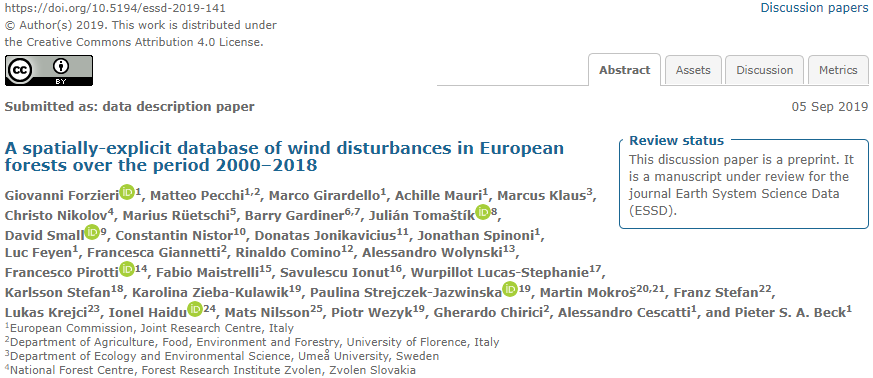
\includegraphics[scale=0.7]{Wind_disturbances_titre}
\end{flushleft}

\begin{flushleft}
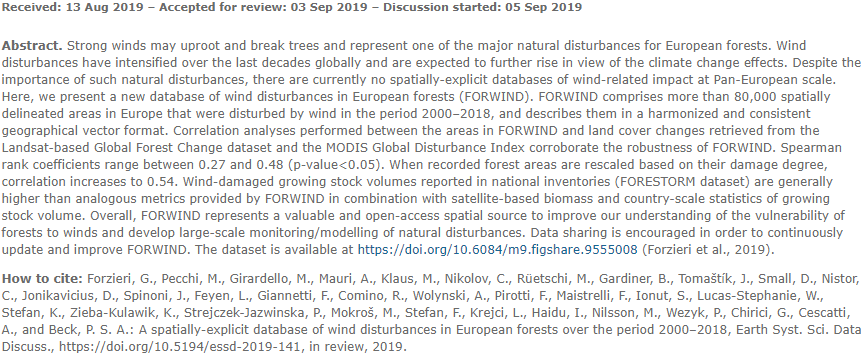
\includegraphics[scale=0.7]{Wind_disturbances_abstract}
\end{flushleft}

\begin{flushleft}
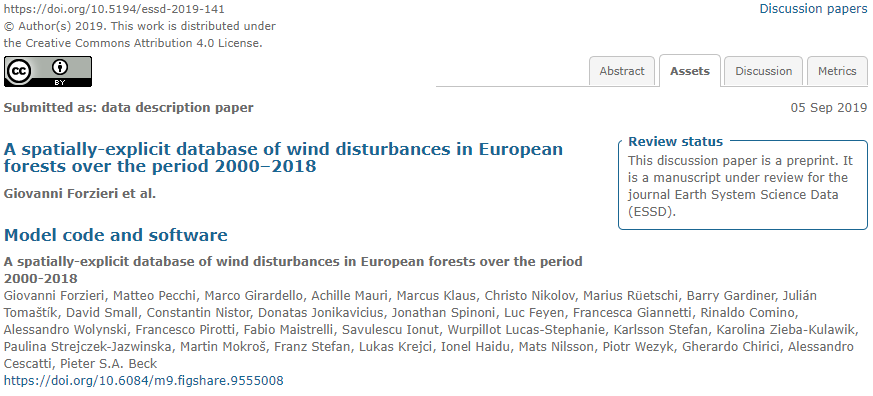
\includegraphics[scale=0.7]{Wind_disturbances_assets}
\end{flushleft}

\begin{flushleft}
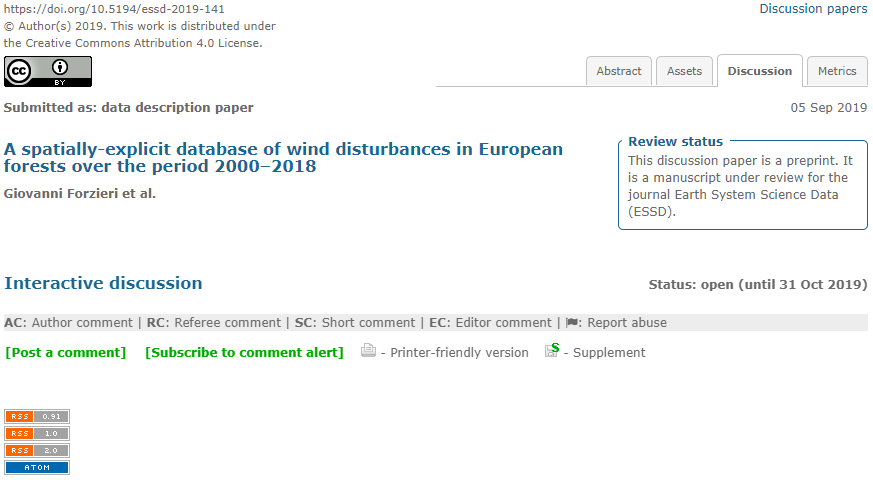
\includegraphics[scale=0.7]{Wind_disturbances_discussion}
\end{flushleft}

\begin{flushleft}
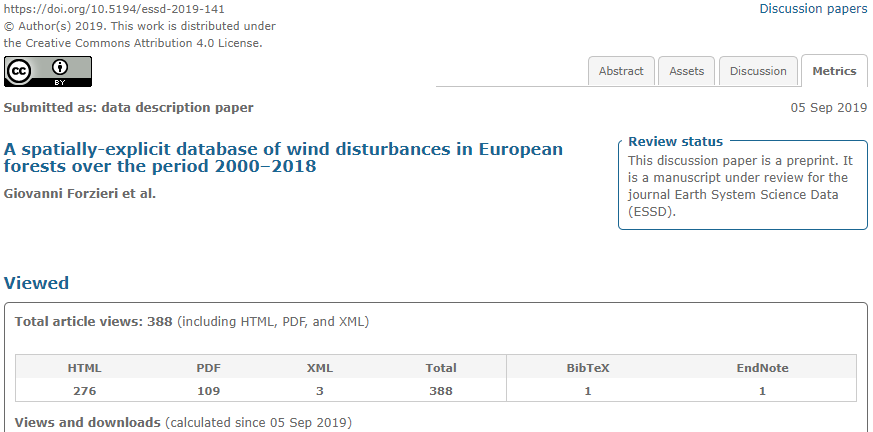
\includegraphics[scale=0.7]{Wind_disturbances_metrics}
\end{flushleft}

\begin{flushleft}
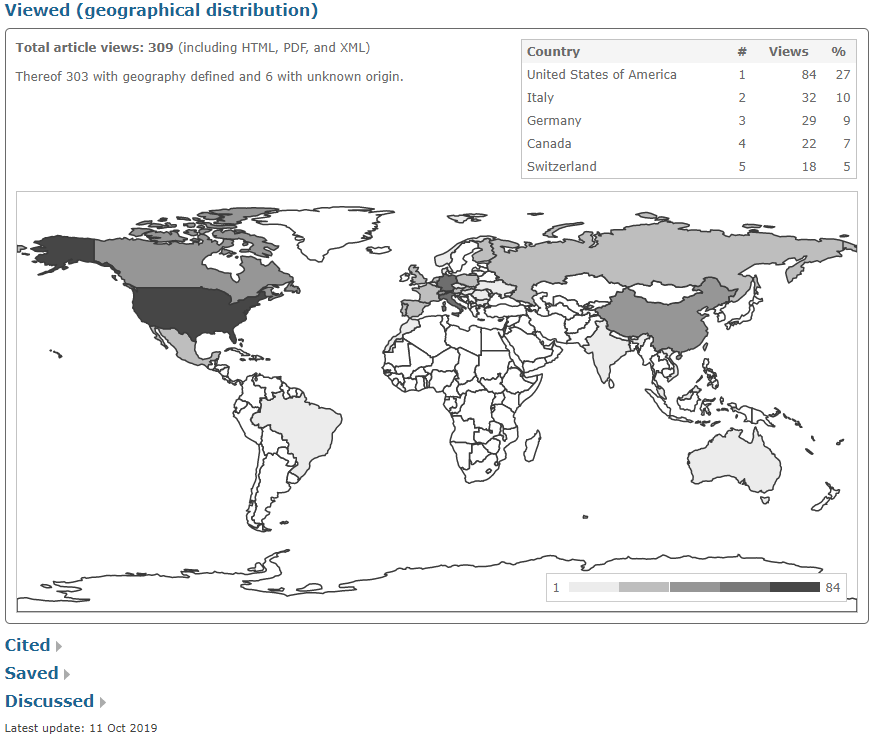
\includegraphics[scale=0.7]{Wind_disturbances_metrics_2}
\end{flushleft}

\begin{flushleft}
Réf : https://www.earth-syst-sci-data-discuss.net/essd-2019-141/
\end{flushleft}

\newpage

\subsection*{Datas papers liés à l'énergie solaire}

...

\section*{Progression sur Github}
- Création d'un dossier partagé

- Familiarisation avec Github et Gitkraken (transfert de fichier, correction ...)


\newpage
\part*{Objectifs pour la semaine prochaine}
\begin{itemize}
	\item Choisir le template du datapaper
	

\end{itemize}


\end{document}